\chapter{Proposed Path Planner}%
\label{chap:proposed_planning}
\textit{Finding a path between the start- and target configuration whilst avoiding collisions with an existing \ac{RRT*} path planner~\cite{chen_fast_2018} was presented at the end of the previous chapter. This chapter extends that existing path planner's configuration space from free- and obstacle space to also incorperate movable- and unknown space. Movable space originates from objects in the environment that are known to be movable, unknown space originates from objects for which it is unknown weither they are movable or unmovable. The planner avoids obstacle space, is incentivezed to plan only in free space but can pass through unknown or movable space. A direct path lies in free space only, a blocked path passes through unknown- or movable space. To free a blocked path and make it a direct path, the object that causes the unknown- or movable space should be moved out of the way. Then a theoretic extension is mentioned to generate paths which respect dynamic constraints.\bs}

\section{Planning in Four Subspaces}\label{sec:planning_in_four_subspaces}
The modified algorithm has four tuning parameters that can be tweaked; The \textit{step size} and \textit{search size} were discussed in \Cref{subsec:path_planning}. The third and fourth tuning parameters are the \textit{UnknownSpaceCost} and \textit{MovableSpaceCost}, which are fixed costs for crossing through unknown or movable space. Crossing through is defined as one or more nodes in the path lying in that subspace. If a path does not contain a node in unknown space, \textit{UnknownSpaceCost} will be 0, equivalent to movable space and \textit{MovableSpaceCost}. These cost are added to the $\mathit{Cost_{path}}$, which is redefined as:\bs

\[\mathit{Cost_{path}} = \mathit{MovableSpaceCost} + \mathit{UnknownSpaceCost} + \sum_{i=1}^{n-1} \mathit{Distance}(\gls{c}_i, \gls{c}_{i+1})\]

Where $\mathit{n} \geq 2$ configuration points make up the path starting at $\gls{c}_\mathit{start}$ and ending at $\gls{c}_\mathit{target}$.\bs

The \ac{RRT*} algorithm searches for a path with the lowest cost, by adding a penalty for crossing through unknown or movable space the path planner is incentivised to find the shortest path around objects but prefers moving an object over making a large detour. Tuning the additional fixed cost for a path crossing through movable or unknown space balances the robot's decision between the length of a detour the robot is willing to drive, compared to pushing an object to free the path. Removing an unknown object bears more uncertainty than a movable object, motivating a higher cost to remove an unknown object compared to an known object. The pseudocode from \Cref{pseudocode:proposed_rrt_star_all} is presented again, with changes due to the extension indicated with a red colour.\bs

\newpage
\begin{algorithm}[H]
  \caption{Pseudocode for extended \ac{RRT*} path planning algorithm. Lines that contain changes compared to \Cref{pseudocode:proposed_rrt_star_all} are indicated with the red colour.}%
  \label{pseudocode:modified_proposed_rrt_star}
  \begin{algorithmic}[1]
    \State $\gls{nodesMP} \leftarrow \gls{nodesMP}_{init}$
    \While{\textit{NotReachStop}}
        \State $\gls{nodeMP}_\mathit{rand} \leftarrow \mathit{Sample_{random}}$ \algorithmiccomment{Create, project and validate a new random sample}
      \State $\gls{nodeMP}_\mathit{nearest} \leftarrow \mathit{Nearest(\gls{nodeMP}_{rand}, \gls{nodesMP})}$
      \State $\gls{nodeMP}_\mathit{temp} \leftarrow \mathit{Project(\gls{nodeMP}_{rand}, \gls{nodeMP}_{nearest})}$
      \If{$\mathit{CollisionCheck(\gls{nodeMP}_{temp})}$}
      \State $\gls{nodeMP}_\mathit{new} = \gls{nodeMP}_\mathit{temp}$
      \State $\mathit{Cost_{toInitMin}} \leftarrow +\infty$ 
      \Else
      \State Continue
      \EndIf
      \State $X_\mathit{near} \leftarrow \mathit{NearestSet(\gls{nodeMP}_{new}, \gls{nodesMP})}$ \algorithmiccomment{Find and connect new node to parent node}
      \For{$\gls{nodeMP}_\mathit{near} \in X_\mathit{near}$}
    \State $\mathit{Cost_{temp}} \leftarrow \mathit{CostToInit}(\gls{nodeMP}_\mathit{near}) + \mathit{Distance}(\gls{nodeMP}_\mathit{near}, \gls{nodeMP}_\mathit{new}) + \textcolor{red}{\mathit{ObjectCost}(\gls{nodeMP}_\mathit{near}, \gls{nodeMP}_\mathit{new})}$
      \If{$\mathit{Cost_{temp}}  < \mathit{Cost_{toInitMin}}$}
      \State $\mathit{Cost_{toInitMin}} \leftarrow \mathit{Cost_{new}}$
      \State $\gls{nodeMP}_\mathit{minCost} \leftarrow \gls{nodeMP}_\mathit{near}$
      \EndIf
      \EndFor
      \If{$\mathit{Cost_{toInitMin}} == \infty$}
          \State Continue
      \Else
      \State $\gls{nodesMP}.add(\gls{nodeMP}_\mathit{new})$
      \State $E.\mathit{add}(\gls{nodeMP}_\mathit{minCost}, \gls{nodeMP}_\mathit{new})$
      \EndIf
      \State $\mathit{Cost_{pathMin}} \leftarrow +\infty$ 
      \For{$\gls{nodeMP}_\mathit{near} \in X_{near}$}\algorithmiccomment{\parbox[t]{.6\linewidth}{Check if the newly added node can lower cost for nearby nodes and if a both connectivity trees can be connected}}
      \If{$\mathit{InSameTree(\gls{nodeMP}_{near}, \gls{nodeMP}_{new})}$}
    \If{$\mathit{CostToInit(\gls{nodeMP}_{new})} + \mathit{Distance(\gls{nodeMP}_{new}, \gls{nodeMP}_{near})} +\textcolor{red}{\mathit{ObjectCost}(\gls{nodeMP}_\mathit{new}, \gls{nodeMP}_\mathit{near})} < \mathit{CostToInit(\gls{nodeMP}_{near})}$}
      \State $\mathit{E.rewire(\gls{nodeMP}_{near}, \gls{nodeMP}_{new})}$
      \EndIf
      \Else \algorithmiccomment{Add lowest cost path to the list of paths}

      \State $\mathit{Cost_{temp} \leftarrow CostToInit(\gls{nodeMP}_{new}) + Distance(\gls{nodeMP}_{new}, \gls{nodeMP}_{near})} + \mathit{CostToInit(\gls{nodeMP}_{near})}$
      % \State $\mathit{Cost_{temp} \leftarrow CostToInit(\gls{nodeMP}_{new}) + Distance(\gls{nodeMP}_{new}, \gls{nodeMP}_{near})} + \mathit{CostToInit(\gls{nodeMP}_{near}) + \textcolor{red}{ObjectCost(\gls{nodeMP}_{new}, \gls{nodeMP}_{near})}}$
      \If{$\mathit{Cost_{temp}  < Cost_{pathMin}}$}
      \State $\mathit{Cost_{pathMin}} \leftarrow \mathit{Cost_{temp}}$
      \State $\mathit{\gls{nodeMP}_{pathMin} \leftarrow \gls{nodeMP}_{near}}$
      \EndIf
      \EndIf
      \If{$Cost_{pathMin} == \infty$}
      \State Continue
      \Else
      \State $\mathit{P.addPath(\gls{nodeMP}_{new}, \gls{nodeMP}_{pathMin}, Cost_{pathMin})}$
      \EndIf
      \EndFor
    \EndWhile
  \end{algorithmic}
\end{algorithm}

The proposed algorithm prevents planning a path through blocking objects except when no other option is available or a large detour can be prevented. No performance tests have been conducted on the modified path planner, apart from visual inspection. \Cref{fig:mp_push_or_drive} clearly shows the effect of varying \textit{UnknownSpaceCosts}.

\begin{figure}[H]
    \centering
    \begin{subfigure}{\textwidth}
    \centering
  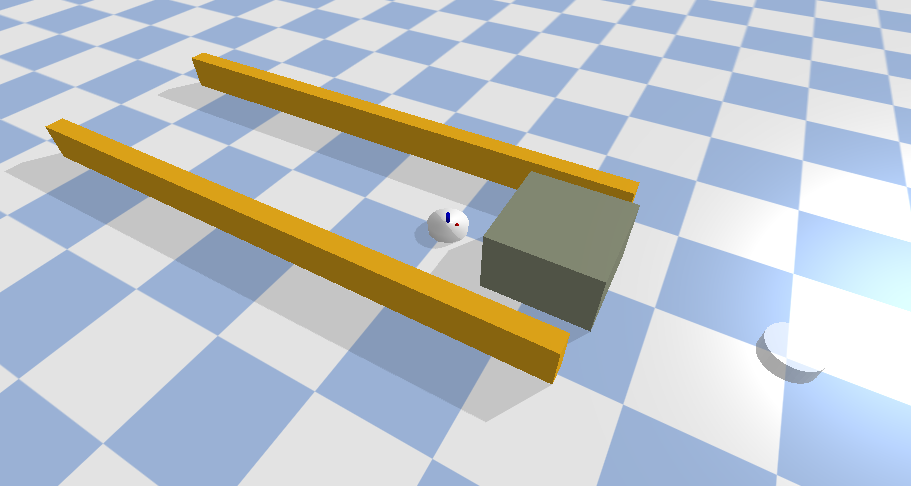
\includegraphics[width=0.8\textwidth]{figures/proposed_method/push_or_drive}
    \caption{Robot environment with the point robot, two yellow unmovable walls and an unknown brown box.\\The robot tasked to drive toward the opposite side of the brown box.}\label{subfig:push_or_drive_env}
    \end{subfigure}

    \begin{subfigure}{1.11\textwidth}
    \centering
    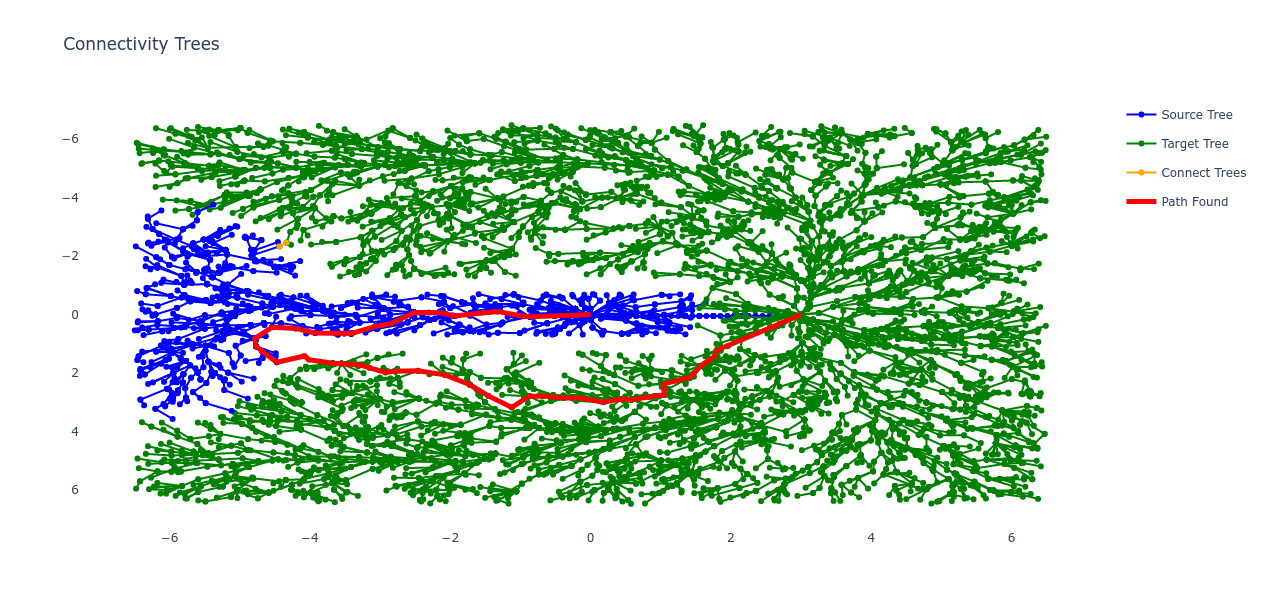
\includegraphics[width=\textwidth]{figures/required_background/mp/mp_high_fixed_cost}
    \caption{Visualization of the planned path around the brown box and yellow obstacles, with $\mathit{UnknownSpaceCost} = 1$.}
    \end{subfigure}

    \begin{subfigure}{1.11\textwidth}
    \centering
    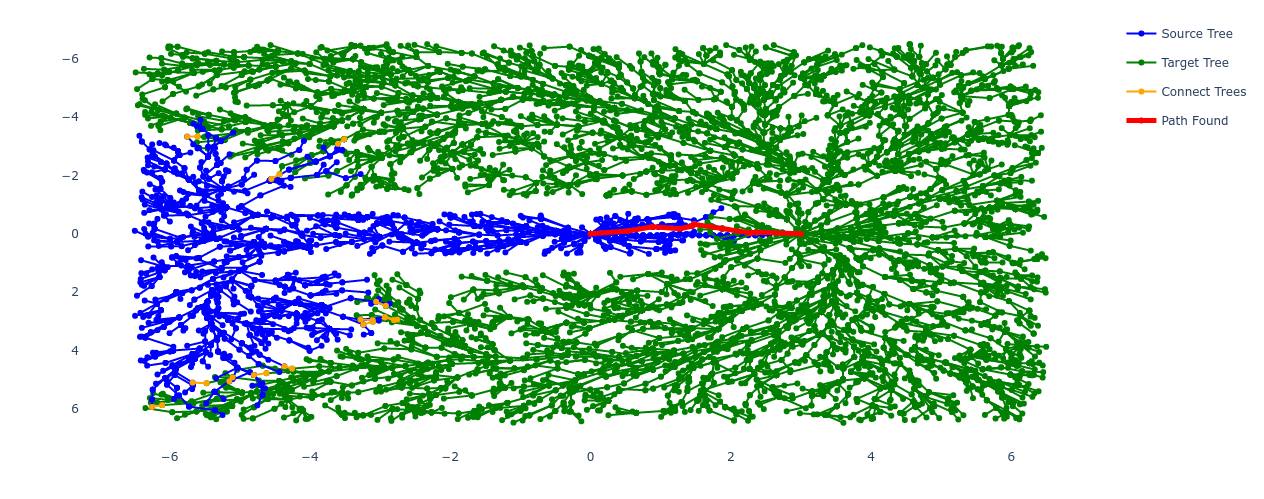
\includegraphics[width=\textwidth]{figures/required_background/mp/mp_low_fixed_cost}
    \caption{Visualization of the planned path going through the brown box, $\mathit{UnknownSpaceCost} = 0.5$.}
    \end{subfigure}
    \caption{Driving task and two planned paths.}%
    \label{fig:mp_push_or_drive}
\end{figure}

\section{Kinodynamic Planning}\label{sec:kinodynamic_planning}
Path planning whilst respecting dynamic constraints (e.g. non-holonomic constraints or constrains on the derivatives of the planned path) is known as kinodynamic planning~\cite{donald_kinodynamic_1993}. A non-holonomic robot, such as the boxer robot in \Cref{subfig:example_boxer_robot} should respect the dynamic constraints, thus a path to track for the robot should be provided by a kinodynamic planner. To take dynamic constraints into account, a dynamic model should be incorporated. The popular method is to use motion primitives~\cite{sakcak_samplingbased_2019,karaman_samplingbased_2011}. Whilst other methods to respect dynamical constraints during path planning do exist (solving a two-point-boundary problem~\cite{li_asymptotically_2016}, setting curvature constraints with a steering function such as Dubins path or Reeds-Shepp curves~\cite{lavalle_planning_2006}) a description is provided to incorporate a dynamic model using motion primitives in the upcoming paragraph.\bs

When sampling a new node in the path planner a dynamic model can be incorporated. Currently a new node is created by generating random number within the boundaries of every dimension of the configuration space. Then to project that configuration point to the closes node, followed by a check if the newly sampled configuration does not lie in unmovable space, see lines 3-11 in \Cref{pseudocode:modified_proposed_rrt_star}. To involve a dynamic model newly samples nodes are created by selecting a existing node, propagate a dynamic system model for a predefined number of time steps using randomly sampled input and the existing node as initial state. If the simulated future state does not lie in unmovable space, it is converted to a newly sampled node for the path planner. That new node, will respect the dynamic constraints since it is is created as a future simulation using a system model that respects the dynamic constraints.\bs

This thesis focuses on the improvement of task execution as a result of learning dynamical models on how to manipulate objects in the robot environment. The proposed path planning algorithm can be extended into a kinodynamic planning algorithm to generate paths that respect non-holonomic and dynamic constraints. As will become clear later in this thesis, the selection of a dynamic model for a certain manipulation action will improve over time when the robot becomes more experienced in the robot environment. To incorporate a system model into path planning leads to the conclusion that: \textit{When using dynamic models that improve modeling the system in term of capturing dynamics and lowering model mismatch, the path planner that incorporates a dynamic model to generate new nodes will improve the paths generated. Where path improvement implies firstly, that the system can be controlled to track a path found, secondly paths that do not respect the dynamic constraints are not generated.} Later in this thesis, during testing, the holonomic point robot is used. Since the point robot has no dynamic or non-holonomic constraints that must be respected, no extension of the proposed planning algorithm is made that makes the path planner a kinodynamic path planner.\bs

Now that the modified path planner is discussed, the proposed robotic framework can be discussed. The proposed framework relies on the required background from previous chapter, and relies on the modified path planner from this chapter.\bs

% old manipulation section shit

% \subsection{Manipulation Planning}%
% \label{subsec:manipulation_planning}
% With a push, two objects are primarily involved, the pushed object and the robot. Generally, and in this thesis, the pushed object's configuration is more important than the robot's configuration. The robot is only a means to push the object toward the target configuration. At which final configuration the robot itself ends up is of lesser importance. As long as during the push, the robot does not collide with objects other than the pushed object, and constraints on the robot must be respected.\bs

% To plan a path that respects the constraints, \todo{Corrado: What does this mean? ->} the robot's configuration is generated for every newly added sample in the manipulation planning algorithm.

% \todo{Gijs For reachbailbpcheck, These lines just point out the name of the function again , there is no added information }
% The \textit{ReachabilityCheck()} (see \Cref{table:functions_for_proposed_rrt_star} and line 33 in \Cref{pseudocode:proposed_rrt_star}) generates the robot configuration to validate if a new sample is reachable from an existing sample. This additional configuration is stored to create only feasible paths that respect the applied constraints. When the stopping criteria are reached and the shortest path is found, the generated robot configurations are discarded. \Cref{fig:manipulation_plannig_local_planner} displays a visual example of the procedure.\bs

% \begin{figure}[H]
%     \centering
%     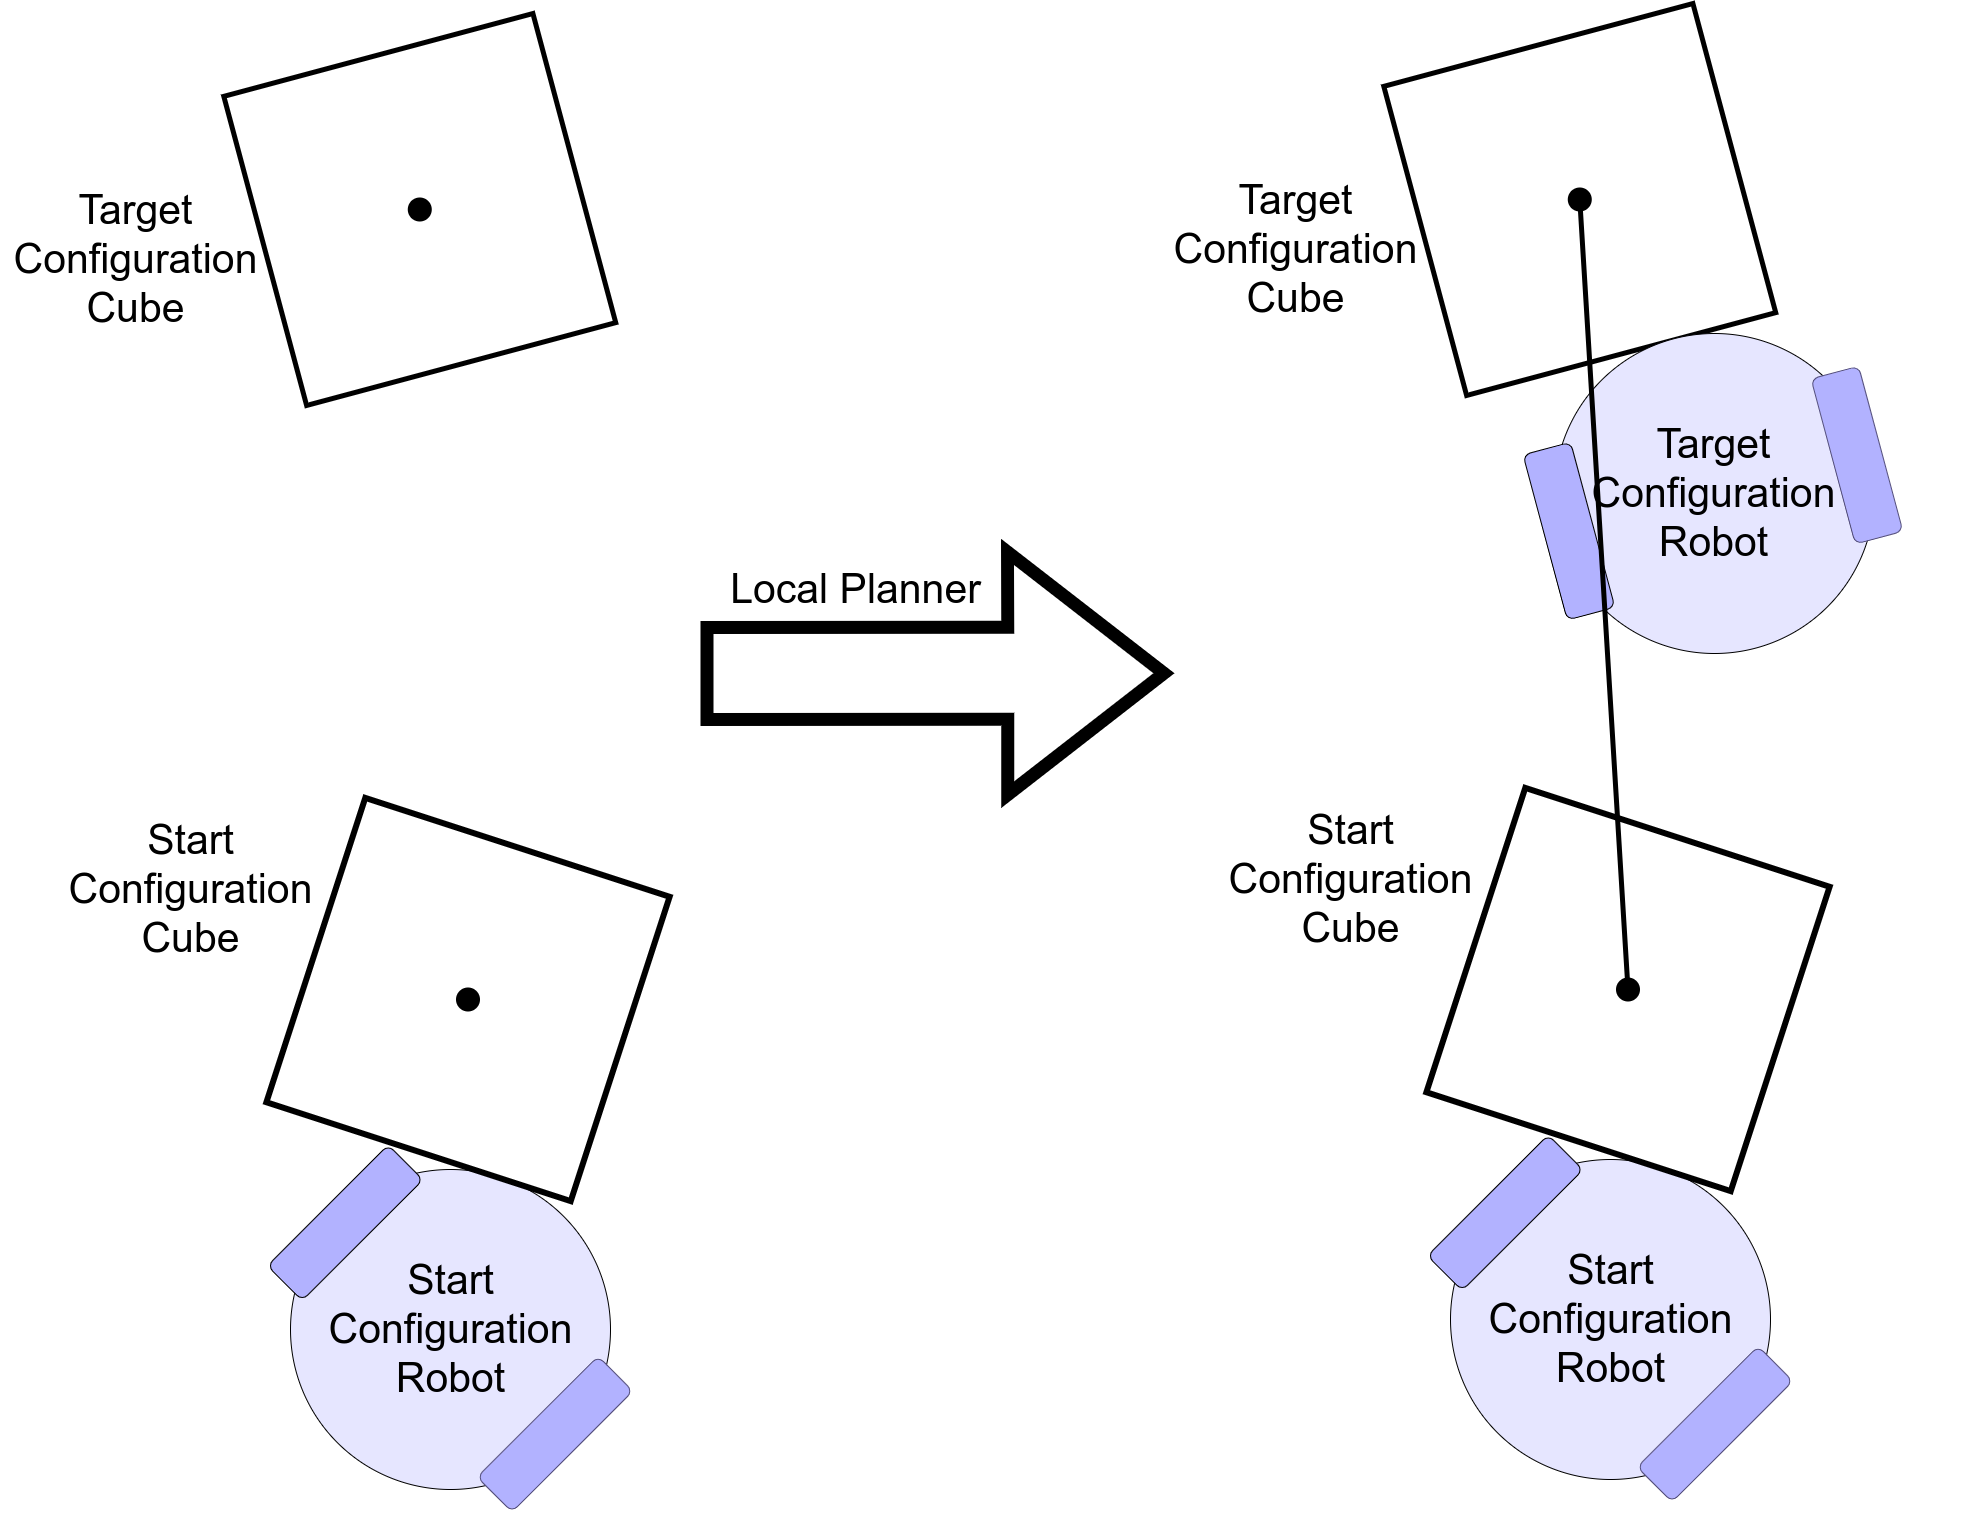
\includegraphics[width=0.6\textwidth]{figures/required_background/manipulation_local_planner}
%     \caption{Generating a new robot configuration whilst adding a sample to the connectivity tree during manipulation planning.}%
%     \label{fig:manipulation_plannig_local_planner}
% \end{figure}
